\section{Assignment Part A}
\label{sec:assignment_part_A}

In this section, we provide a brief overview of the requests associated with the first part of the assignment, along with a description of the approach taken to fulfill them.
Discussion of the results obtained is also included.



\subsection{Request}
\label{subsec:request_part_A}

Starting from the data collected in the provided \texttt{rosbag} file, the goal of this first part of assignment is to evalute at each time instant, the following quantities:

\begin{itemize}
    \item \textbf{Minimum distance} of the vehicle from the obstacles in the environment;
    \item \textbf{Estimate of \texttt{/cmd\_vel} command} sent to the vehicle during the simulation.
\end{itemize}

We also recal that the \texttt{rosbag} file was obtained by running a \texttt{Turtlebot3} robot of the model \texttt{burger} in a simulated environment, specifically the \texttt{turtlebot3\_world} provided by the \texttt{turtlebot3\_gazebo} package.

\begin{figure}[H]
    \centering
    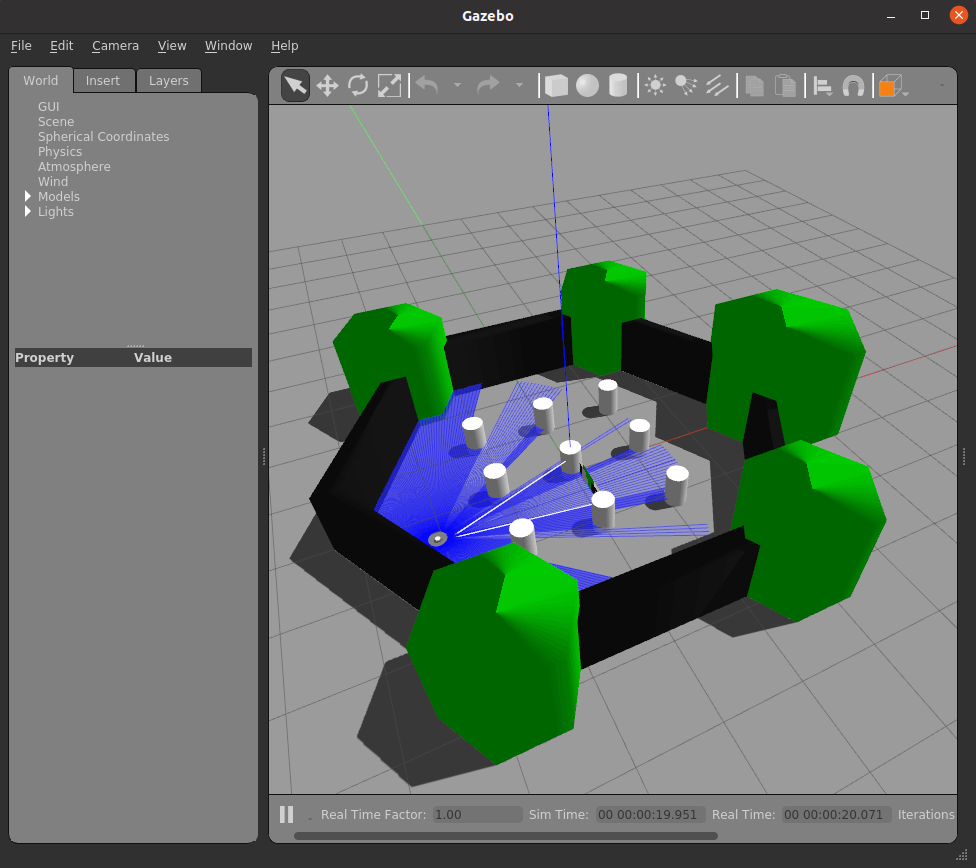
\includegraphics[width=0.6\textwidth]{./img/gazebo_world.png}
    \caption{Gazebo world used for the simulation. Credit to \url{https://emanual.robotis.com/}}
    \label{fig:turtlebot3_world}
\end{figure}



\subsection{Analysis}
\label{subsec:analysis_part_A}

At first, the \texttt{rosbag} file is loaded into \texttt{MATLAB} using the \texttt{rosbag} function, which allows to read and manipulate \texttt{rosbag} files in a convenient way.
A preliminary analysis of the data contained in the \texttt{rosbag} file is performed showing the following topics:

% \begin{lstlisting}[
%     style=Matlab-editor,
%     caption={Topics contained in the \texttt{rosbag} file.},
%     label={lst:rosbag_topics}
% ]
% bag = rosbag('bags/provided.bag');
% bag.AvailableTopics
% \end{lstlisting}

% Which returns the following topics:

\begin{table}[H]
    \centering
    \begin{tabular}{l|l|l}
        ~      & \textbf{NumMessages} & \textbf{MessageType}   \\
        \hline
        /clock & 110,710              & rosgraph\_msgs/Clock   \\
        /imu   & 110,240              & sensor\_msgs/Imu       \\
        /odom  & 3,316                & nav\_msgs/Odometry     \\
        /scan  & 552                  & sensor\_msgs/LaserScan \\
        /tf    & 3,316                & tf2\_msgs/TFMessage    \\
        \hline
    \end{tabular}
    \caption{Topics contained in the \texttt{rosbag} file.}
    \label{tab:rosbag_topics}
\end{table}


\subsubsection{Minimum distance from obstacles}
\label{subsubsec:minimum_distance}

Given the presence of the \texttt{/scan} topic, which contains the laser scan data, we can use it to compute the minimum distance from obstacles in the environment.
The \texttt{scan} message contains a field called \texttt{ranges}, which is an array of distances measured by the laser scanner at different angles.
The minimum distance can be computed by taking the minimum value of this array, which represents the closest obstacle detected by the laser scanner at that time instant.
The following code snippet shows how to extract the \texttt{ranges} field from the \texttt{/scan} topic and compute the minimum distance at each time instant:

\begin{lstlisting}[
    style=Matlab-editor,
    caption={Extracting the \texttt{ranges} field from the \texttt{/scan} topic and computing the minimum distance at each time step.},
    label={lst:minimum_distance}
]
scan = select(bag, 'Topic', '/scan');
scan_msgs = readMessages(scan, 'DataFormat', 'struct');
scan_time = scan.MessageList.Time - scan.StartTime;
scan_ranges = cell2mat(cellfun(@(msg) msg.Ranges(:)', scan_msgs, 'UniformOutput', false));
min(scan_ranges, [], 2)
\end{lstlisting}

One can also plot the minimum distance over time, as shown in Figure \ref{fig:minimum_distance}.

\begin{figure}[H]
    \centering
    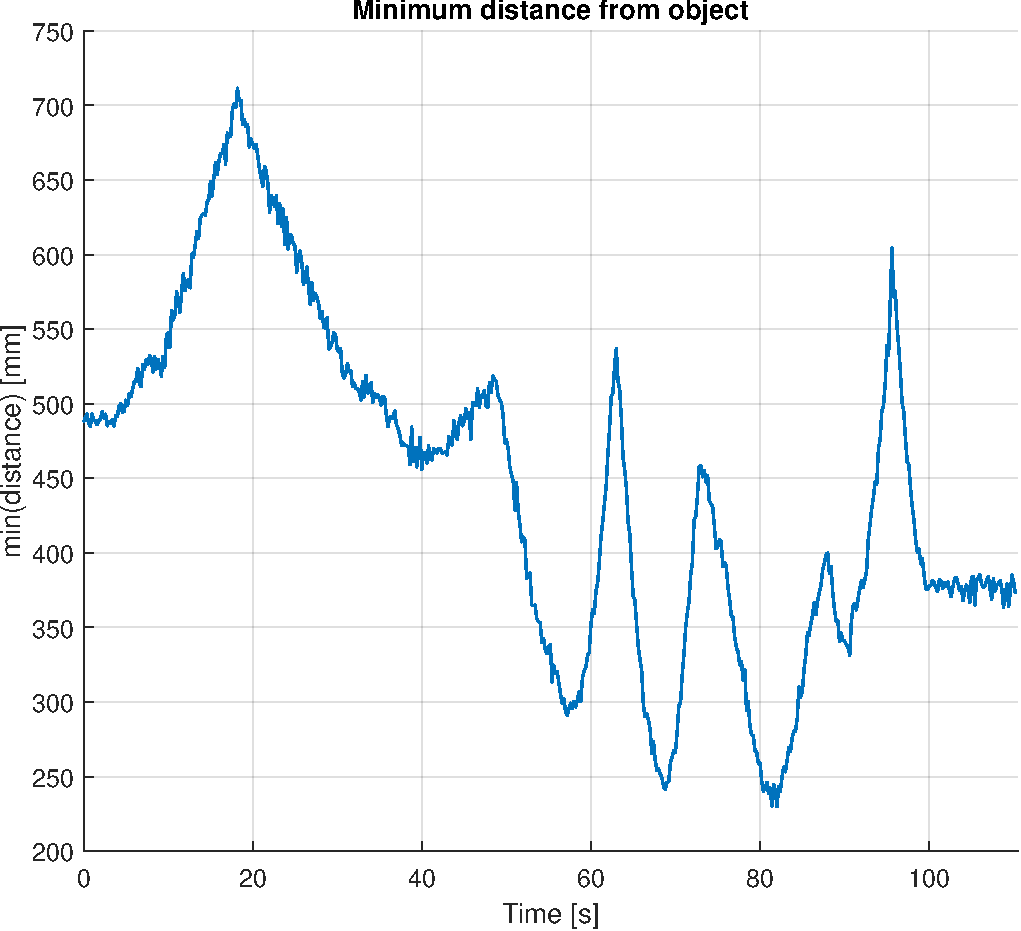
\includegraphics[width=0.7\textwidth]{./img/MATLAB/minimum_distance.pdf}
    \caption{Minimum distance from obstacles over time.}
    \label{fig:minimum_distance}
\end{figure}

It's important to notice that, being the data coming from a simulated environment, we can expect the accuracy of the laser scanner to be almost perfect (unless the simulation environment add noise on purpose), while on a real vehicle we could face issues like sensor noise or hit of minimum and/or maximum range of the laser scanner.
This could lead to a less accurate estimation of the minimum distance from obstacles, which could be a problem for the robot navigation and obstacle avoidance.


\subsubsection{Estimate of \texttt{/cmd\_vel} command}
\label{subsubsec:cmd_vel}

The \texttt{/cmd\_vel} topic usually contains the velocity commands sent to the robot, which are typically represented as linear and angular velocities.

As an exercise, given that in the provided \texttt{rosbag} file the \texttt{/cmd\_vel} topic has been removed, we can estimate the linear and angular velocities of the robot using the \texttt{/odom} topic, which contains the odometry data.
The \texttt{odom} message contains the position and orientation of the robot in the world frame, as measured by the odometry system.

Again, with a similar faschion as done for the \texttt{/scan} topic, we can extract the information from the \texttt{/odom} topic, save them in a matrix form and plot them.

\begin{figure}[H]
    \centering
    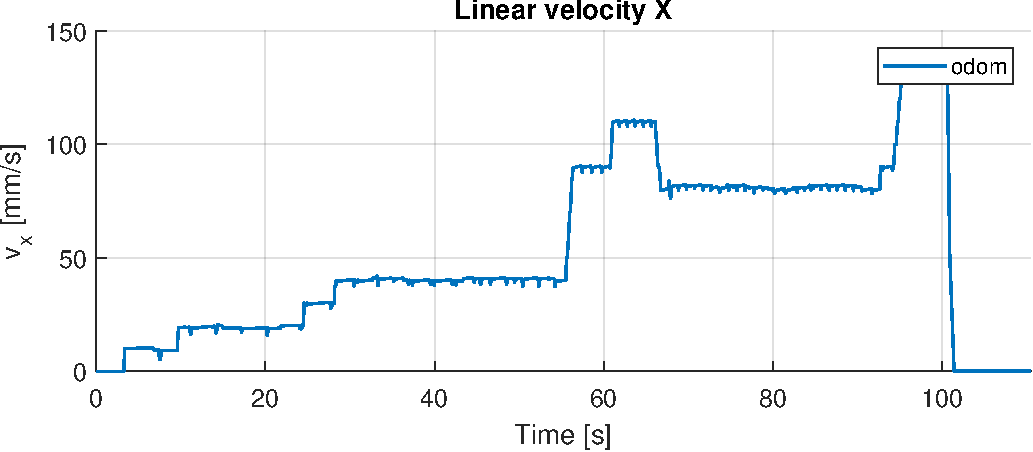
\includegraphics[width=0.8\textwidth]{./img/MATLAB/linear_velocity.pdf}
    \vspace{9pt}
    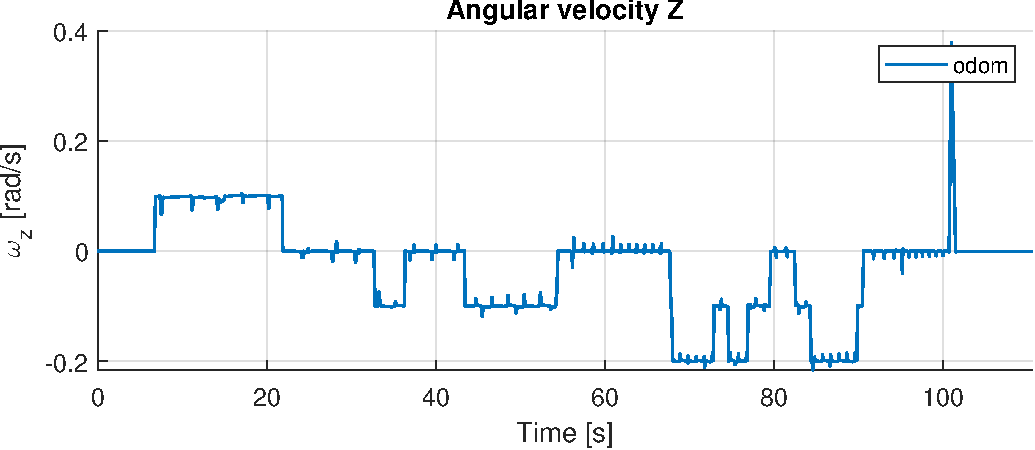
\includegraphics[width=0.8\textwidth]{./img/MATLAB/angular_velocity.pdf}
    \caption{Velocities of the robot over time, purerly based on the odometry data.}
    \label{fig:odom_velocities}
\end{figure}

Notice that one could have also possibly used the \texttt{/imu} topic to estimate both position and velocities of the robot (via single and double integration of the acceleration data).
However, due to the presence of noise in the IMU data and cumulative errors due to integration, this approach is definitely not recommended as it easily results in drifted output estimation.

On the other hand, a sensor fusion approach based for example on the Kalman filter could have been used to combine the two sources of data (IMU and odometry) ultimately increasing the overall accuracy.

